%\chapter{sciencetech}

%%%%%%%%%%%%%%%%%%%%%%%%%%%%%%%%%%%%%%%%%%%%%%

% \section{Overview}

The DUNE primary physics program focuses on long-baseline neutrino oscillation physics, nucleon decay and supernova burst and 
astro-physics \cite{dunecdr} and plans to employ a 40 kton LAr detector underground. The protoDUNE program will make 
measurements to significantly enhance the reach of DUNE in each of these areas. 
In addition, some protoDUNE measurements of hadronic interaction on Ar nuclei will be the first of their kind 
and hence are expected to be significant results in their own right. 




% Describe what parameters are relevant for various physics measurements
% * beam\\
% * NDK\\
% * atmospherics\\
% * SN physics\\
% �> some of interest as standalone measurements

The DUNE sensitivity assumes a significant advance in a reduction of various sources of uncertainties. In table \ref{tab:DUNEsen} the list of collated sources of uncertainties compared with the lists for MINOS and T2K $\nu_e$ appearance analyses are presented. 
%
\begin{cdrtable}[DUNE goals are for the total normalization uncertainty on the $\nu_e$ appearance sample.] {ccccc} {DUNEsen} {DUNE goals are for the total normalization uncertainty on the $\nu_e$ appearance sample. The DUNE analysis will be a 3-flavor oscillation fit such that uncertainties correlated among the four FD samples will largely cancel \cite{cdr-vol-2}.}
Source of Uncertainty &  MINOS $\nu_e$ & T2K $\nu_e$ & Goal for DUNE $\nu_e$  \\ \toprowrule
 Beam Flux                        &  0.3\% & 3.2\%  &  2\%&  \\ \colhline
Interaction Model               & 2.7 \%  & 5.3\% & ~2\%  \\ \colhline
Energy Scale ($\nu_\mu$) &  3.5\% & included above  &  (2\%) included in  \\
					 &   &   &   5\% $\nu_\mu$ uncertainty  \\ \colhline
Energy Scale ($\nu_e$)     & 2.7\% & 2.5\% includes all FD effects &  2\% \\ \colhline
Fiducial Volume                 & 2.4\% & 1 \% & 1\%  \\ \colhline
Total Uncertainty                & 5.7\% & 6.8\% &  3.6\%  \\ \colhline
\end{cdrtable}
%
To achieve this reduction of uncertainties, a program of measurements is needed using various detectors. ProtoDUNE-SP will be particularly useful to measure detector effects with full-scale components as planned for the DUNE far detector and a long drift volume. 

While long-baseline physics studies are not sufficiently advanced to establish firm requirements on individual systematic parameters or detector effects the studies conducted to date indicate 
that energy scale measurements at the single particle level, efficiencies for calorimetry and background rejection, especially e-gamma 
separation are of particular interest. From the DUNE long-baseline physics perspective the goal of the protoDUNE measurements program 
should be the validation of detector simulations and measurement techniques such that these may be applied in the DUNE far detector environment.

Nucleon decay searches aim to discover or alternatively set a lower limit on the lifetime for specific decay processes. The lower limit 
on the partial lifetime is described by equation \ref{eqn:ndk_limit}
\begin{equation}
\tau/B = \frac{n_{p/n} \varepsilon M t} {N_{obs} - N_{backgr}} \,\,\, ,
\end{equation}
where  $\tau/B$ is the (lower limit on the) partial lifetime sensitivity (in yr).
On the right hand side of the equation
$n_{p/n}$ is the number of protons or neutrons per unit mass (in 1/kton ), $\varepsilon$ is the signal detection efficiency, $Mt$ is the detector exposure (in ton yr) and $N_{obs} - N_{backgr}$ is the (upper limit on the) number of signal events.

ProtoDUNE measurements will affect $\varepsilon$ and $N_{backgr}$ through 
particle identification performance and track and shower reconstruction performance measurements as well as
pion and kaon cross section measurements on Ar nuclei.
In addition, experimental data may 
help to refine the nucleon decay event selection in a LAr TPC which is equivalent to the DUNE far detector.

The study of atmospheric neutrinos in DUNE allows measurement of the mass hierarchy and oscillation parameters including 
a unitarity test by means of the tau neutrino appearance channel.  For atmospheric neutrino interactions simulation studies indicate that 
typically 1 to 5 hadrons are expected in the final state. While neutrino induced hadronic showers will be different from those produced by 
single particles in a test beam, the same nuclear models used for both types of interactions can be validated
Furthermore, reducing the angular and energy resolution for single hadrons and multi-particle hadronic systems is expected to lead 
to better mass hierarchy sensitivity. Measurements of and improvements to particle identification and pion and kaon interactions on Ar nuclei 
will improve the overall uncertainty of measurements relevant for atmospheric neutrinos.


For SNe neutrinos the relevant energy range of tens of MeV is significantly lower than what can be studied with charged particles at the H4 
beamline. However, stopping muons originating from the beam and from cosmics and associated Michel electrons will allow to study the 
detector response in the relevant energy range. In particular, the light yield of the photon detection system in response to Michel electrons 
will be of interest to evaluate PDS trigger efficiencies for SNe neutrinos. Stopping muons and Michel electrons also serve as low energy 
calibration sources and planned studies are described in that context in section \ref{sec:calibration}.


The following sections describe the planned studies sub-divided into measurements on the hadronic and electromagnetic systems
and measurements focused on the evaluation of event reconstruction and particle identification performance.

%%% For lepton energy resolution and energy scale uncertainty we would need to measure differences between particles and antiparticles and any nonlinear effects.  

%%% For hadronic energy resolution and energy scale uncertainty, there will be different contributions from different particles types (protons, neutrons, charged pions, neutral pions) in different portions of the neutrino spectrum. 
%%% One of the most important measurements will be a determination of the missing/undetected energy. 

%%%Below we provide a list of the main ProtoDUNE-SP studies that will be performed using charged particles from the beam and particles created by cosmic muons. The studies will inform us about the detector response to particles/tracks/showers that will be observed in the neutrino-induced events in the DUNE detectors. 


\section{Hadronic physics topics}
incoming primaries:  pion, proton: 1- few GeV

Accurate measurement of neutrino energy will require characterisation of both electromagnetic and hadronic showers. Reconstruction of hadron energy in these energy ranges will require knowledge of the fate (interact, decay, or stop) of the initiating hadron ($\pi^{+/-}$, $p$, or $K^{+/-}$).
For the case of interacting hadrons, the composition of secondaries
will need to be determined to characterise the response. 
These will include neutrals and particles that deposit energy electromagnetically ($\pi^o$, $\gamma$), as well as
secondary hadrons. The test beam with known incoming particle type and momentum will be used
to characterise interacting hadrons in this energy range.



\subsection{Energy scale}

for different shower complexities

%%%--- \item [Characterization of hadronic showers (high $p$) and topologies of hadronic interactions (low $p$).]



Figure~\ref{fig:hadronshwr} shows the fraction of true energy deposited by interacting protons with 1~GeV/c (left) and
3~GeV/c (right) incident momenta simulated using FLUKA particle transport code~\cite{fluka05}. 
Interacting protons (65\% of the 1~GeV/c sample) are selected.
For this study, visible energy is summed using hit information with corrections applied for the lifetime of the drift electrons (No attempt is made to correct for recombination effects or electromagnetic shower fractions). 
The resulting energy deposition in the two cases cannot be accurately characterized by an average shower calibration factor. MC simulations of outgoing particles, especially at low energies, must be checked and benchmarked against calibration data to avoid significant uncertainties from shower modeling. 

\begin{cdrfigure}[Fraction of true energy deposited by interacting protons of 1~GeV/c and
3~GeV/c]{hadronshwr}{Fraction of true energy deposited by interacting protons of 1~GeV/c (left) and
3~GeV/c (right) momenta simulated using FLUKA~\cite{fluka05}.}
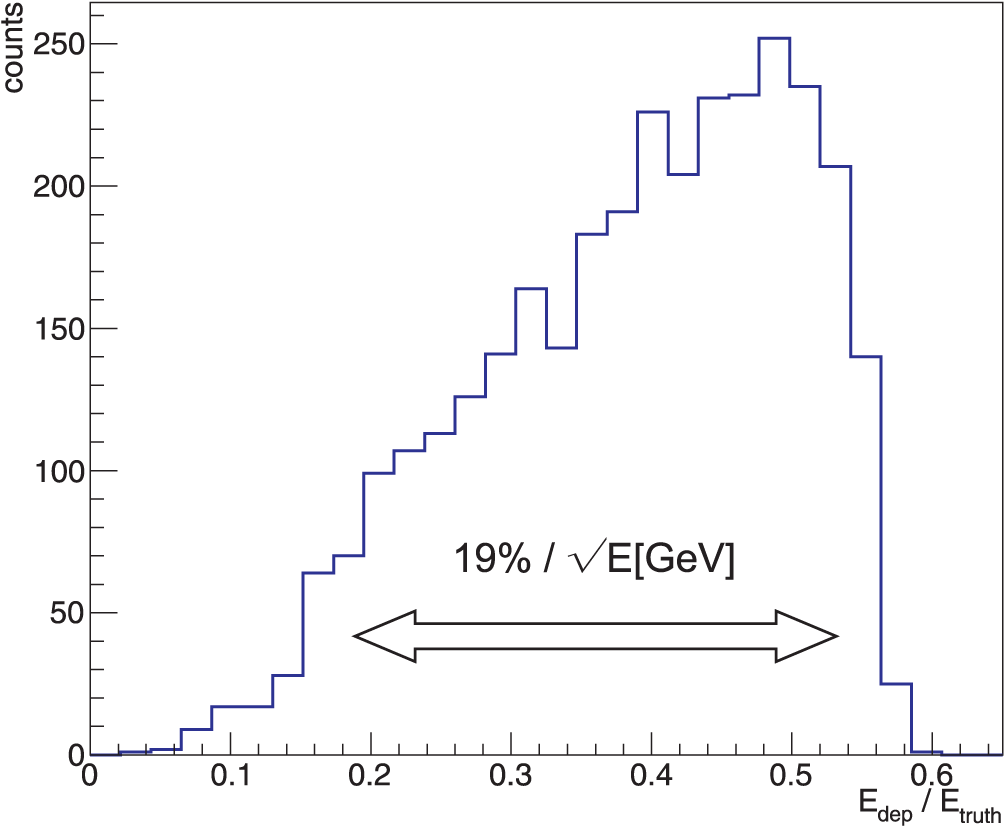
\includegraphics[width=0.49\textwidth,height=5.0cm]{pr1GeV_v2a}
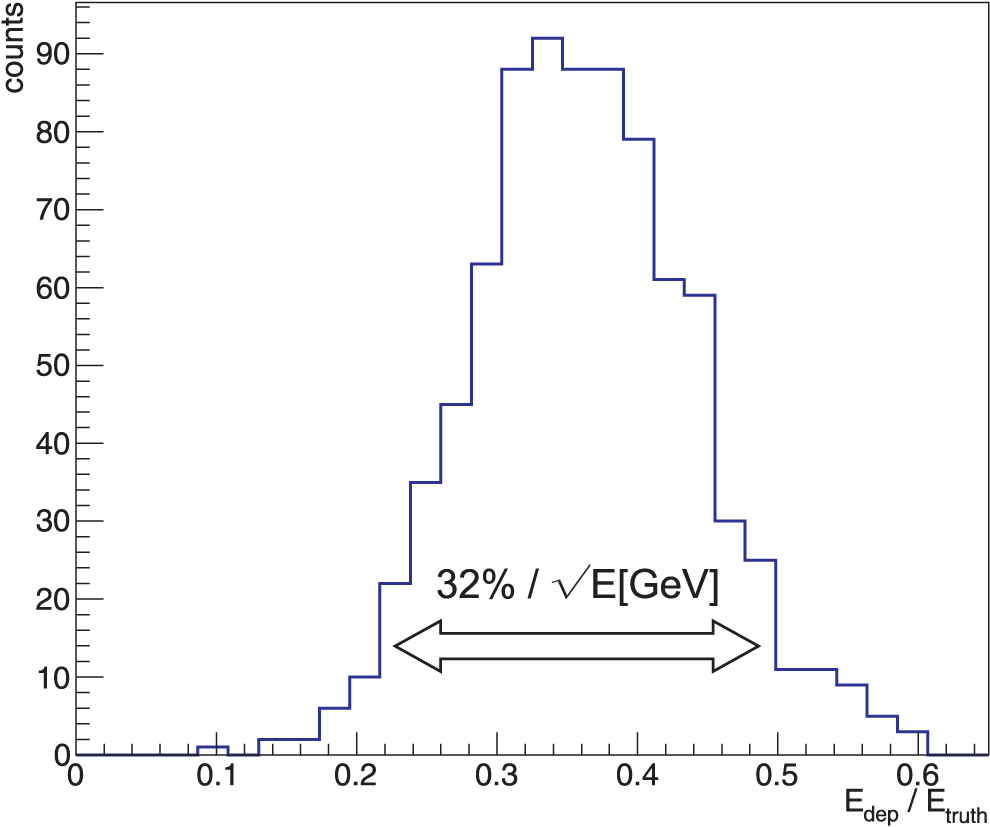
\includegraphics[width=0.49\textwidth,height=5.0cm]{pr3GeV_v2a}
\end{cdrfigure}


Pion showers at low energies will also be important both for determining the interacted neutrino energy and for modelling neutral current backgrounds resulting from $\pi^o$ content in showers. Significant differences in energy deposited in interactions initiated by $\pi^+$ versus $\pi^-$  are present up to momenta of an order of 1~GeV/c due to different final-state particles and interaction cross sections. This is illustrated in  Figure~\ref{fig:pionshwr}, which shows the differences in mean energy deposited (left) and width (right)  for interacting pions with momenta ranging from 0.2~GeV/c up to 5~GeV/c.
Resulting shower calibrations and reconstruction will differ; therefore each charge must be studied separately. This study will be performed if a low momenta run will take place.  

\begin{cdrfigure}[Differences in mean energy deposited and width of visible energy, 
 $\pi^+$ versus $\pi^-$]{pionshwr}{Differences in mean energy deposited (left) and width of visible energy (right) 
for interacting $\pi^+$ versus $\pi^-$ ranging from 0.2~GeV/c up to 5~GeV/c. }
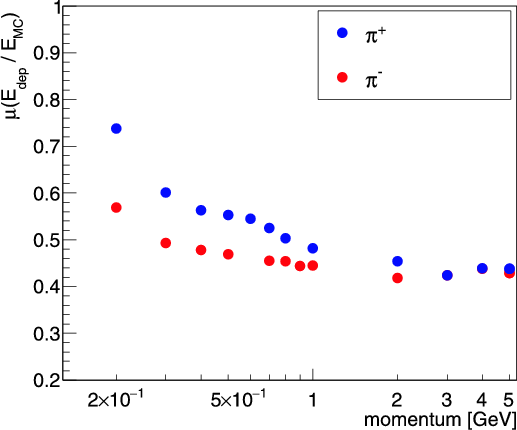
\includegraphics[width=0.49\textwidth,height=6.0cm]{pipimean_ticks1}
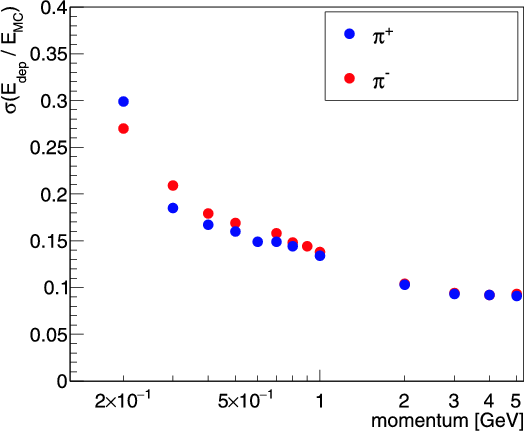
\includegraphics[width=0.49\textwidth,height=6.0cm]{pipisigma_ticks1}
\end{cdrfigure}




\paragraph{Missing energies}
	     
	     The measured energy deposition for various particles and its dependence on the direction of the particle will be used to tune
MC simulations and allow improvements to the reconstruction of neutrino energy and interaction topologies. 
Measurements of the response to charged particles and photons with the protoDUNE-SP will extend and be complementary to
measurements made with other smaller detectors, such as LArIAT \cite{lariat}.
 LAr TPC enables the use different energy reconstruction methods. 
 %In particular, in LAr TPC we can infer $E_\nu$ from what we observe in the final state. 
 ArgoNeuT neutrino energy reconstruction method included estimates of missing/invisible energy, and important part of the improved neutrino energy reconstruction included the measurement of neutrons. 
 Precise and unbiased neutrino energy reconstruction is especially important for reducing systematics in precision neutrino oscillation experiments. The systematic uncertainty which creates a bias in neutrino energy measurement  affects the ability to precisely measure oscillation parameters.  The inclusion of neutrons in the estimation of neutrino energy improves energy resolution from 14\% to 3\%
 \fixme{need reference}.  
 Due to its large size protoDUNE-SP has the ability to measure protons that are created via the neutron-proton charge exchange process.
 Hence it allows to validate the accuracy of missing energy fractions as predicted by MC simulations and thereby improve the uncertainty on the 
 energy bias.

	     
\subsection{Studies of e.m. fractions}

 (as function of primary hadron energy)
	
	
\subsection{Multiplicities in hadronic interactions}
 (pi0 and others)

\subsection{Shower topologies}


\subsection{Shower development}
  (energy deposition mechanisms)\\
	  �> verification of MC models

	
\subsection{Cross section measurements}
 (exclusive + total hadronic)\\
		(absorption, charge exchange, inelastic, elastic, �)\\

Detailed knowledge of pion-nucleus cross sections in the sub-GeV energy range is required to tune generators~\cite{genie} to model event visible energy accurately. 
Existing data used to tune the models cover limited energies ($<$200~MeV) and are primarily on lighter target nuclei~\cite{fsirev}.
The requested $\pi^+$ and $\pi^-$ samples will allow new data samples for measuring
exclusive final state processes of $\pi^+$ and $\pi^-$ over the full relevant \fixme{quantify} energy range and specifically on argon nuclei. 
The H4 beam line will allow to collect $\pi^+$ and $\pi^-$ data with momenta above\,1~GeV/c.  
Synergies with the LArIAT experiment will be explored to investigate agreement within the overlapping energy region.  A high-statistics sample of charged particles will allow precise measurements of charged mesons' interaction cross sections and particularly various exclusive channels.


\paragraph{Pion interactions}
		
		Final state pions are produced copiously in neutrino interactions in the energy range for the DUNE beam  and contribute 
substantially to the total visible energy in the interaction.
Pions can re-interact either in the nuclear medium or after emerging from the target nucleus
and significantly change the visible energy deposited in the event. 
The importance of modeling final-state pion interactions on reconstructed neutrino energy has been recently demonstrated in the NuMI, and Booster beam energy ranges~\cite{miniboonefsi, minervafsi}. The results from Minerva and MiniBoone are in tension and even more sophisticated final state interaction models cannot resolve the disagreement. 



\paragraph{Resonance production}
	 
\subsection{Pi-zero production model tests}

\subsection{Kaon interactions}
 rare in beam line but numerous from pion interactions in side detector\\ 
	       �> kaon decay\\
		==> p-decay sensitivities\\

%%%--- kaon interaction cross section to remove proton decay backgrounds

The DUNE experiment in the deep underground location will seek to detect several modes of proton decay.
%In particular, a first ever LAr detector 

This first-ever LAr detector of this scale underground will primarily improve sensitivity to proton decays with final state kaons such as  ${p \rightarrow K^+ \overline{\nu}}$. 
Sensitivity to this process is studied in~\cite{bueno}. $K^+$ detection efficiency is estimated to be $>$97\% in the
appropriate momentum range (500-800 MeV/c). The kaon samples needed for this study might not be available in the H4 beam line, as most of the kaons will decay before reaching the protoDUNE detector. 

To provide the needed 2000 stopping $K^+$ track samples for the PID studies, a sample of 13k beam kaons with 1~GeV/c momentum must be obtained (Only 15\% of $K^+$ stop at 1~GeV/c.), which will likely be difficult in this beam line. 
A sizable sample of protons ($\sim 10^6$) is also needed. This will allow a study of the possible background contributions to $p \rightarrow K^+ \overline{\nu}$ to quantify the probability of an interacting proton being misidentified as stopping kaon. A proton interaction that produces neutrals and one charged pion 
(that is misidentified or subsequently decays to $\mu$) can fake the final-state kaon signal.




\section{Electromagnetic physics topics}

%Electromagnetic showers are relatively well-understood and can be used to understand the detector response better. 
The beam of electrons will be studied at various energies to characterize the induced showers.

Decays of neutral pions induced in the interactions of hadrons in the beam at one to few GeV/c momentum
will be used as a source of photons producing electromagnetic showers at a broad range of angular orientations.
This sample will be used to validate techniques for electromagnetic showers separation from the hadronic
component of the event. Such techniques are a prerequisite for the use of the generic EM shower reconstruction
algorithms (see section ~\ref{sec:larsoftreco}), and in particular for studies of energy scale calibration
based on neutral pion invariant mass reconstruction. Also, hadronic shower energy estimation, as mentioned
in the previous section, requires splitting between electromagnetic showers and hadronic tracks. Finally,
test beam event topologies with $\pi^0$ production are similar to those expected in neutrino events, and
will be studied as described in the following section.


	\subsection{Electron shower}

		\paragraph{Energy resolution}
		 (at higher energies)

		\paragraph{Energy scale}

	\subsection{e/gamma separation}
	
	The search for a CP violation phase using $\nu_e$ appearance 
in a $\nu_\mu$ beam requires good electron/photon separation.
Backgrounds originating from photons produced primarily from final state $\pi^0$'s must be identified and removed from the signal
electron sample. 

High-energy photons can undergo two processes: pair production and Compton scattering. 
The dominant process for photons with energies of several hundred MeV or more is 
e$^+$ e$^-$ pair production.
For this process e/$\gamma$ discrimination can be achieved using the beginning of the electromagnetic shower, where a single MIP is characteristic of electron energy deposition, while two MIPs would be consistent with e$^+$ e$^-$ pair production. 


\begin{cdrfigure}[Photon background rejection versus electron identification efficiency for various energies]{egam}{Photon background rejection versus electron identification efficiency for various energies( 100 MeV - 5 GeV for photons and 100 MeV - 2 GeV for electrons), calculated for and normalized to samples which pass the reconstruction.  The simulation was performed in APA design configuration (4.67-mm wire pitch, induction wires at $\pm$35.7$^{\circ}$ w.r.t. collection wires).}
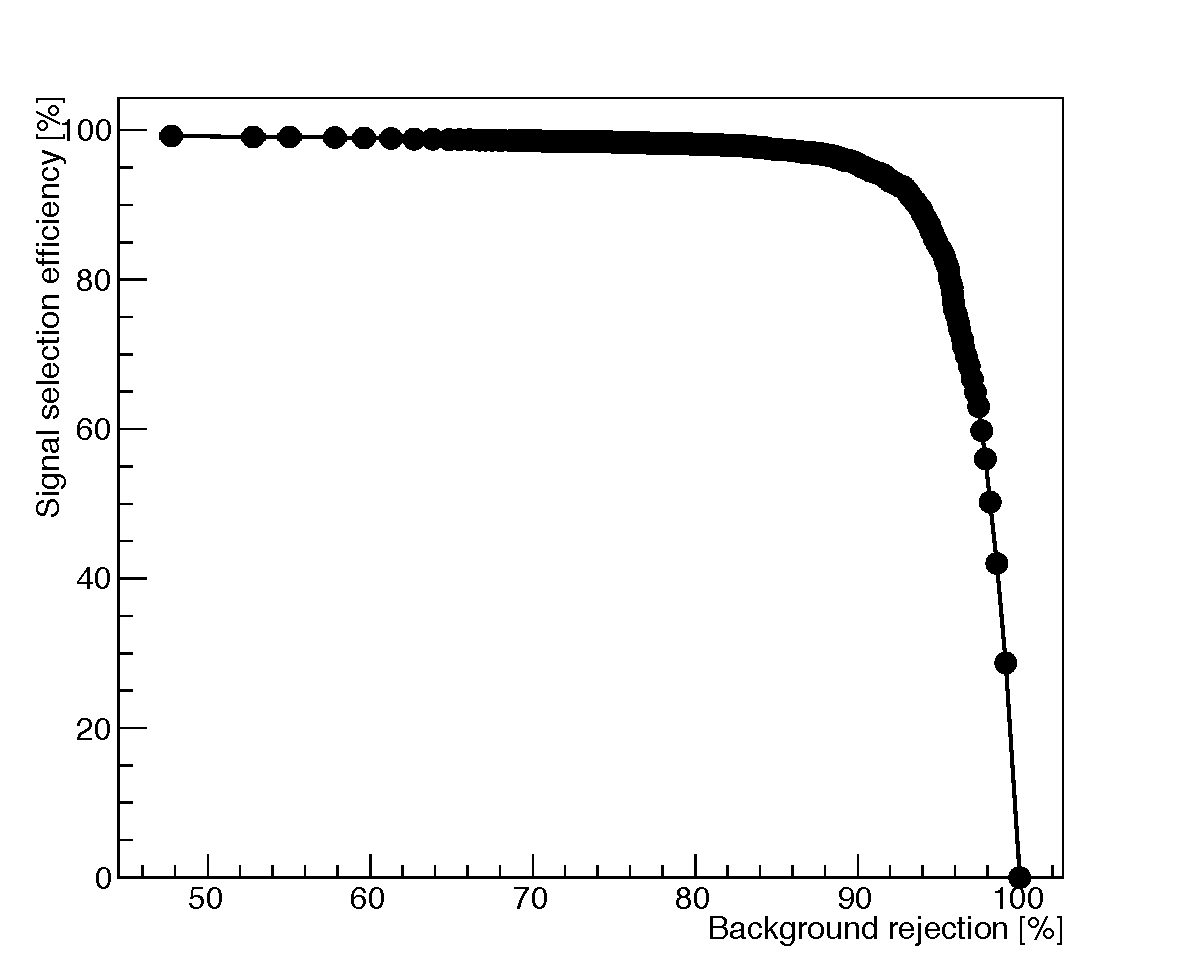
\includegraphics[width=0.5\textwidth,height=6.0cm]{egammaeffbkg}
\end{cdrfigure}


Electron-photon separation has been studied in LArTPCs  detectors that collected data in recent years (ICARUS~\cite{icarus_eg} and ArgoNeuT~\cite{argoneut_eg}).

Figure~\ref{fig:egam} shows estimated photon background rejection versus electron identification efficiency using simulated isotropic electron and photon event samples with the DUNE APA geometry configuration (4.67-mm wire pitch,
induction wires at $\pm$35.7$^{\circ}$ w.r.t. collection wires).~\cite{dunecdr}. The study was performed on the
simulation of isolated particles to separate from the present state of the art of pattern recognition algorithms
and their inefficiencies. Instead, the unavoidable features, such as an overlay of signals from multiple tracks in the
interaction vertex region, was mimicked with the parameterized subtraction of information from the initial part of
simulated cascades.

The results are found to be mildly dependent on incoming particle energy in the range of interest. 

Pure samples of electrons and photons in the sub-GeV energy range would be required to tune the separation algorithms and to measure detector-dependent electron-photon separation efficiency and purity. 
Such an idealistic conditions cannot be easily achieved with the test beam, but charged pion interactions might be very well studied to evaluate performance of the background rejection based on the observation of double m.i.p. and (or) photon-induced cascade displacement from
the interaction vertex.

	
	\subsection{Charge identification via muon capture}

With non-magnetized LArTPC detectors, it is not possible to determine particle charge on an event-by-event basis. Therefore, a statistical separation that makes use of differences in muon versus antimuon capture cross sections and lifetime will be investigated.
About 99.9\% of $\mu^-$'s are expected to be captured on argon, compared to essentially all $\mu^+$ to decay ~\cite{stopmu}.
Charge-sign tagged $\nu_\mu$ samples, which predict differences in the particle and antiparticle survival probabilities, may be useful for constraining exotic possibilities, such as non-standard neutrino interactions. 
A well-developed muon tagging would enhance the MH studies for the atmospheric neutrinos. 


\section{Evaluation of event reconstruction and particle identification performance}

	\subsection{Reconstruction algorithm performance test}

		\paragraph{Energy dependency}
		\paragraph{Efficiencies}

	\subsection{Particle Identification}
	
	Information on a range and charge deposition for stopping charged-particles can be used to identify particle type as well as measure kinetic energy accurately. Figure~\ref{fig:resrange}  (left) shows track energy loss per unit length \footnote{Signal attenuation due to recombination effect is not corrected for the PID purpose since it is a deterministic transformation which does not add measurement information.} $dQ/dx$ as a function of residual track range for simulated muon, pion, and proton particle tracks. The sequence of $dQ/dx$ versus residual range reconstructed for a particle track is used as input to PID algorithms ~\cite{nn_pid,rd_pid} to evaluate each particle hypothesis.

Figure~\ref{fig:resrange} (right) shows the distribution of reconstructed $dQ/dx$ in a narrow bin at a residual range of 6($\pm$1)cm to illustrate the scale of difference between particle types. Proton band is well separated from pion and muon bands, while pion and muon bands are almost overlapping which is challenging for the efficient separation via ionization density differences. 
Simulation is performed with LArSoft framework using ProtoDUNE-SP geometry including the beam orientation and GEANT4 based simulation of particle transport through LAr. Parameterization of the detector response is implemented according to the scheme existing in the LArSoft framework, with a dedicated setup for ProtoDUNE-SP conditions. Pattern recognition and 3D reconstruction are performed with Line Cluster and Projection Matching algorithms (one of standard reconstruction schemes currently used for ProtoDUNE).

The PID efficiency and purity depend on a number of factors, such as the detector configuration, geometry and reconstruction algorithms. PID results on data, especially for pion/muon separation, may be significantly different if e.g. electronics noise assumed in the detector response simulation is not reproducing features of the DUNE readout chain or if signal processing and reconstruction algorithms are updated. It is, therefore, important to test entire PID scheme in a prototype detector data, using the presence of all detector effects to improve models used in both simulation and reconstruction. Event samples that include an adequate number of stopping particles for each species
(muon, pions, protons and kaons) are included in the particle summary request to perform tests of PID algorithms and Bethe-Bloch calibration measurements.

\begin{cdrfigure}[ProtoDUNE-SP simulated track $dQ/dx$]{resrange}{ProtoDUNE-SP Simulated track $dQ/dx$ as a function of residual range for muons, pions, protons and kaons, used as training data in a neutral-net-based PID algorithm (left). Distribution of $dQ/dx$ for each particle type for a bin with residual range 
6($\pm$1)~cm (right). The small difference between muon and pion PID is illustrated.}
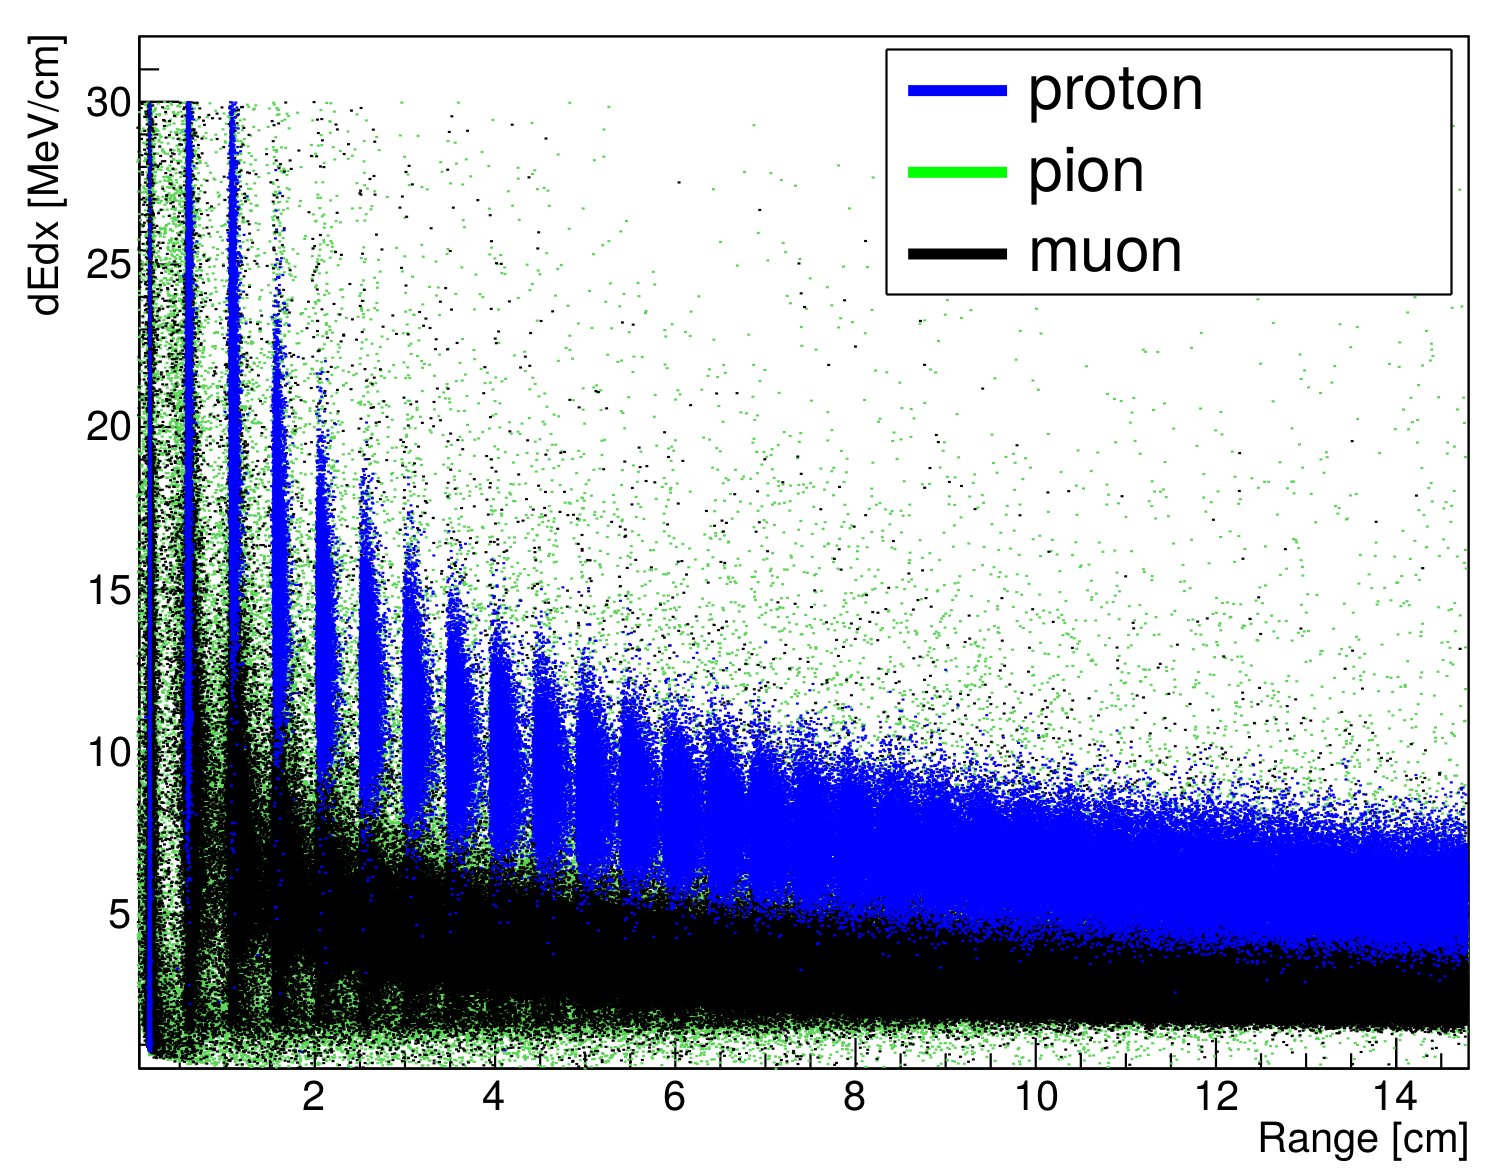
\includegraphics[width=0.53\textwidth,height=6.0cm]{dEdxprmupi}
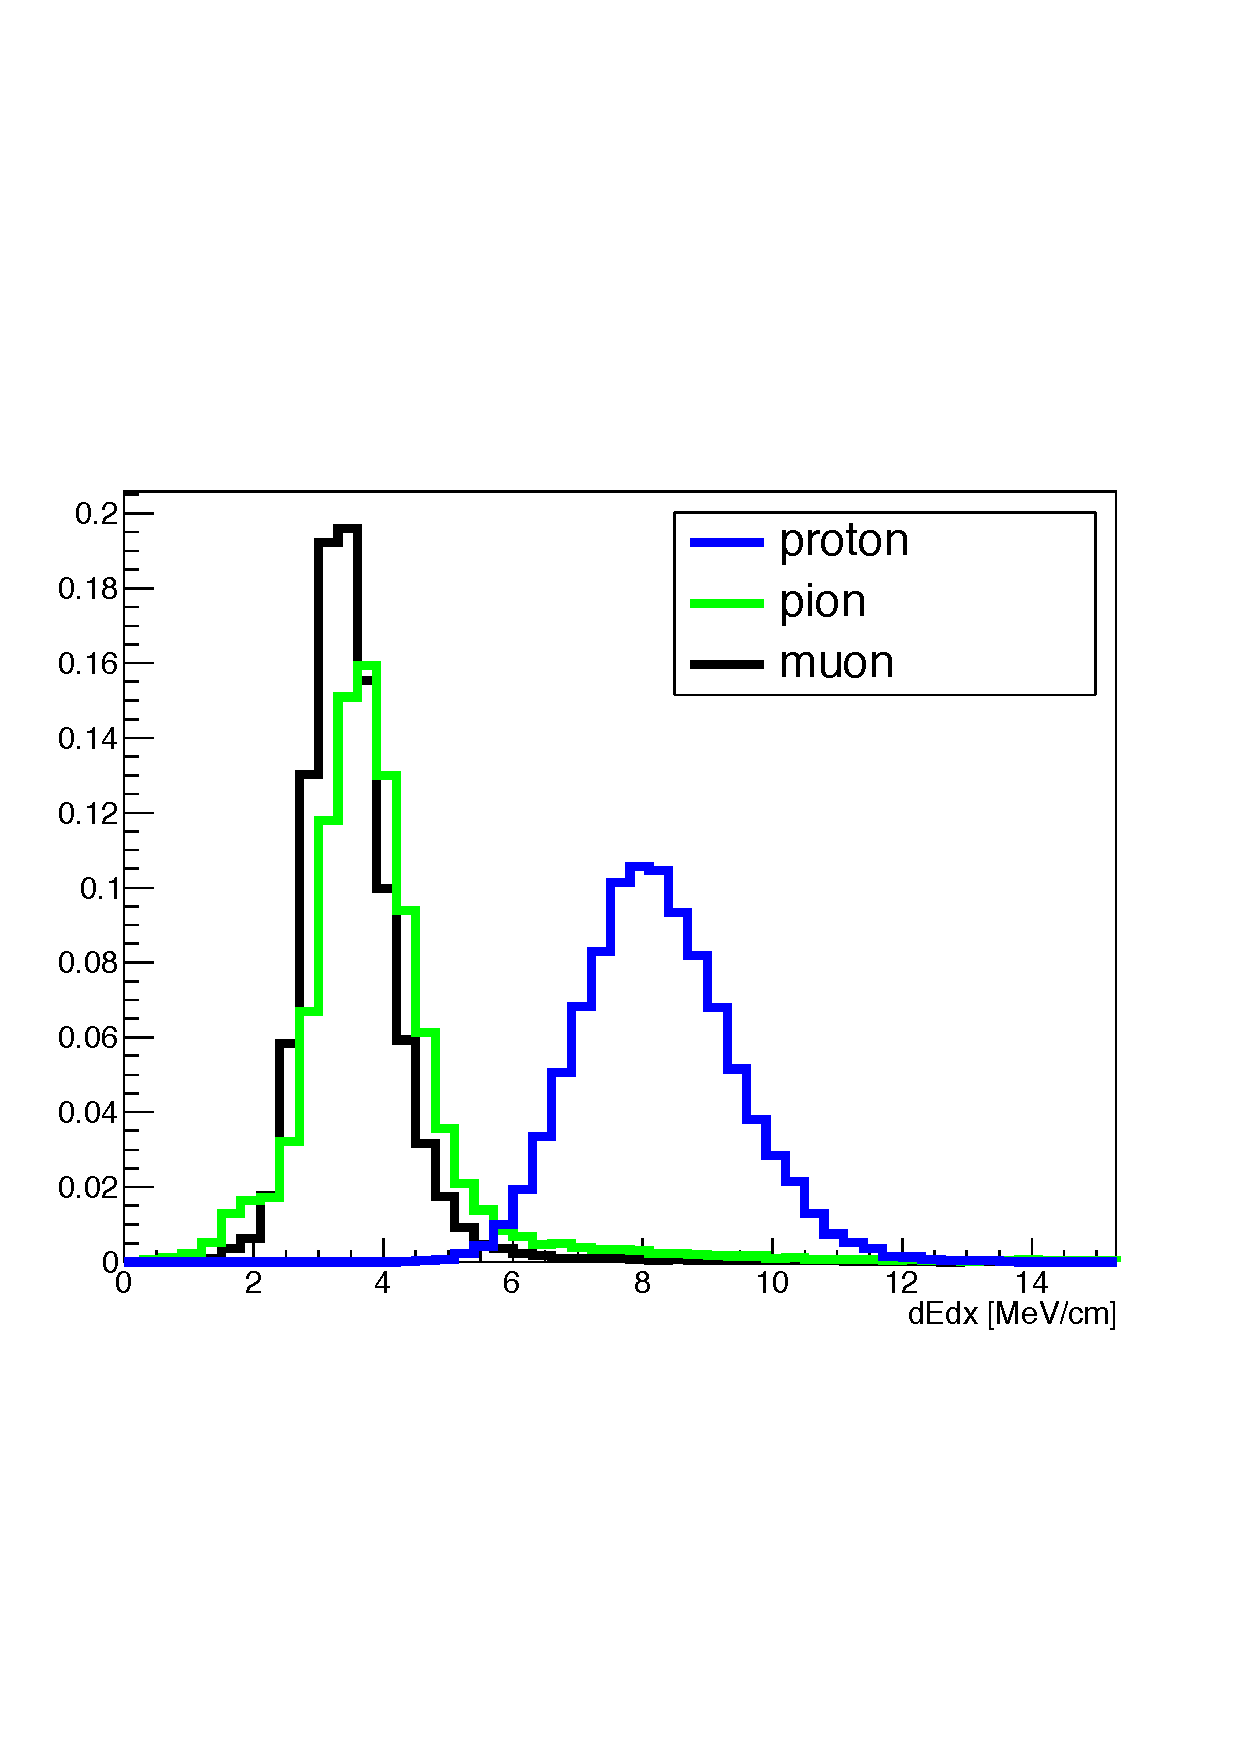
\includegraphics[width=0.46\textwidth,height=6.0cm]{dEdxprmupienbin}
\end{cdrfigure}


		\paragraph{Stopping particles}

		\paragraph{Low energy}

		\paragraph{e/gamma separation}
 	also have this under em physics already ...



%%%%%%%%%%%%%%%%%%%%%%%%%%%%%%%%%%%%%%%%%%%%%%%%%%
\newpage
%%%---\section{Overview}
\fixme{Anne added this section 7/28; there needs to be a general intro. I've borrowed this text from CDR detector vol, sec 9.3.1) }

As an \textit{engineering} prototype, ProtoDUNE-SP is
intended to validate the construction of the components planned for the
first DUNE \ktadj{10} detector module at scale and thereby mitigate
risks associated with extrapolating small-scale versions of the
single-phase LArTPC technology to a full 10-kt detector module.  It is
intended to benchmark the operation of the full-scale detector
elements and perform measurements in a well characterized
charged-particle beam --- an essential step.

The prototype will incorporate components with the same
dimensions and features as those for the first 10-kt DUNE far detector
module.

Besides validating the performance of the detector components,
planning and constructing the protoDUNE-SP prototype will establish and
commission production sites and test the installation procedure.
Further, before the beam test, many primary detector-performance parameters can be established with cosmic-ray muons.  These data will aid in the identification of potentially problematic components, leading to future improvements and optimizations of the detector design.  Once
it is exposed to a test beam of charged particles of different types
and energies it will collect data that can be combined with results from LArIAT and the short-baseline program at Fermilab.  Together
these measurements will be used to validate MC simulations, reduce several detector and cross section and reconstruction uncertainties, and they
will serve as data input to DUNE sensitivity studies and allow
validation and tuning of tools for event reconstruction and particle
identification.

The current plan is to take high-momentum, above 1GeV/c  data with the protoDUNE-SP detector during the first period of data-taking. The total number of trigger that we should be able to collect is about 25 million and will take about six weeks. This will allow collecting enough data to perform all high statistics measurements described below.  If time allows it would also be beneficial to collect data with lower momenta particles. The switch to low momenta run would require modifications of the beam-line instrumentation, removal of several detectors and retune of the magnets. However, the low momenta beam has a significantly lower intensity, and it might be difficult to collect datasets necessary for some of the studies (e.g. Kaons for proton decay background studies).

%%%%%%%%%%%%%%%%%%%%%%%%%%%%%%%%%%%%%%%%%%%%%%
%%%---\section{Charged particle beam studies}
\fixme{Science description?}

The DUNE experiment will run in both neutrino and antineutrino 
configurations. These beams will be composed mainly of muon neutrinos (antineutrinos) as well as electron neutrinos (antineutrinos). With a neutrino beam with a wide neutrino energy range, various types of particles can be produced due to neutrino interactions and re-interactions in the nucleus.  In Figure~\ref{fig:particlemomenta} the momentum distributions particles created in neutrino interactions from simulated beam fluxes, including oscillation effects, are shown.  The particle rates are normalized  to the number of neutrino interactions in the DUNE far detector and the neutrino beam flux.  Although a significant fraction of the final state particles produced in neutrino interactions will have low momenta, due to constrains of the H4 beam and operation time main part of the measurement program will focus on particles with momenta above 1\,GeV/c. There will be an overlap between data and results from protoDUNE-SP and the low momenta LArIAT experiment that will help with the extrapolation to the most interesting low momenta region.  Although the H4 beam can produce low momenta particles, it is at the cost of lower rate of the particles and longer operation time. If the beam is available, the second run with a focus on low momenta particles will be performed. 


\begin{cdrfigure} [Momentum distributions]{particlemomenta}{Momentum distributions of particles produced by the neutrinos from the neutrino beam in DUNE.  Each of the particles leaving the nucleus is show here separately. } 
  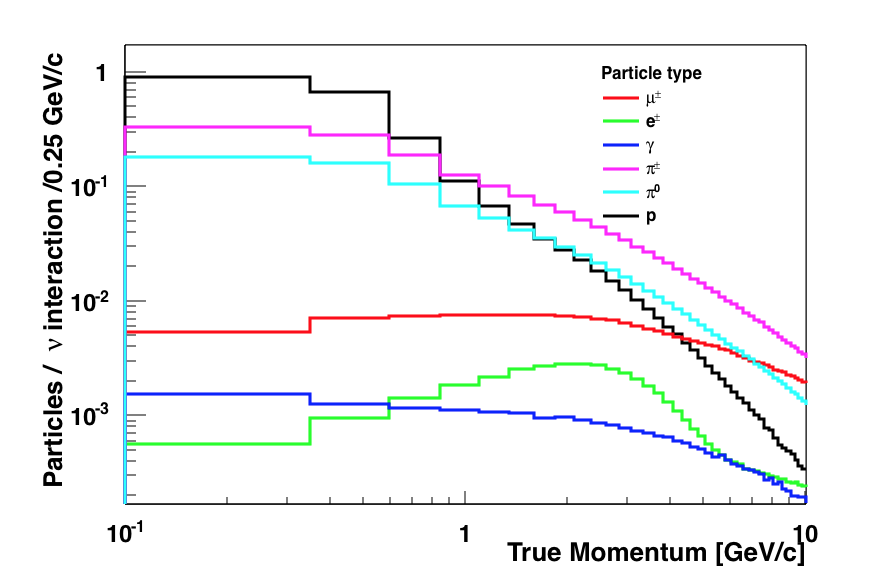
\includegraphics[width=0.8\textwidth]{True_Momenta_per_Particle_9_2_1_0_logy_logx}
\end{cdrfigure}



\begin{description}


\item [Characterization of electromagnetic showers]

\fixme{need more text - RS: adding few more lines on purposes of pi0s, please add more on electrons}


\item [Study of $e/\gamma$ separation capabilities]

%\fixme{Sentence feels unclear; the ``DUNE'' APA configuration? DONE!}



\item [Validate accuracy of MC simulations] 

The accuracy of MC simulations will be validated for relevant energy ranges. Models of the pion, kaon interactions as well as for other hadrons will be checked and measured in the energy range and for argon for the first time allowing reduction of the systematic uncertainties. For the simulation of the charged particles interactions the LArSoft framework with GEANT MC will be used in a similar manner as it will be done for the DUNE simulations. All chains of the simulations and analysis will be prototyped, developed and validated with the protoDUNE-SP simulations and data. 

\end{description}


\fixme{Plots to be generated for  sections 2.1-2.3. Not necessary all of them need to be included in the final version of the TDR.}
\begin{itemize}
\item Containment for charged particles in the ProtoDUNE for the predicted particle beam. 

Figure~\ref{fig:containment} shows the simulated longitudinal and transverse 
energy containment for proton showers up to 10~GeV in energy.
For 10-GeV showers, more than 95\% of the energy is contained in a detector of longitudinal size of 6~m and radius of 2.5~m. Showers from pions, kaons, and electrons have also been studied, and similar or better containment is achieved in these cases, given the above detector dimensions.


\begin{cdrfigure}[Simulated longitudinal and transverse containment for proton showers, 4 and 10~GeV/c]{containment}{Simulated longitudinal and transverse containment for proton showers of 4 and 10~GeV/c momenta.}
  \begin{tabular}{ccc}
   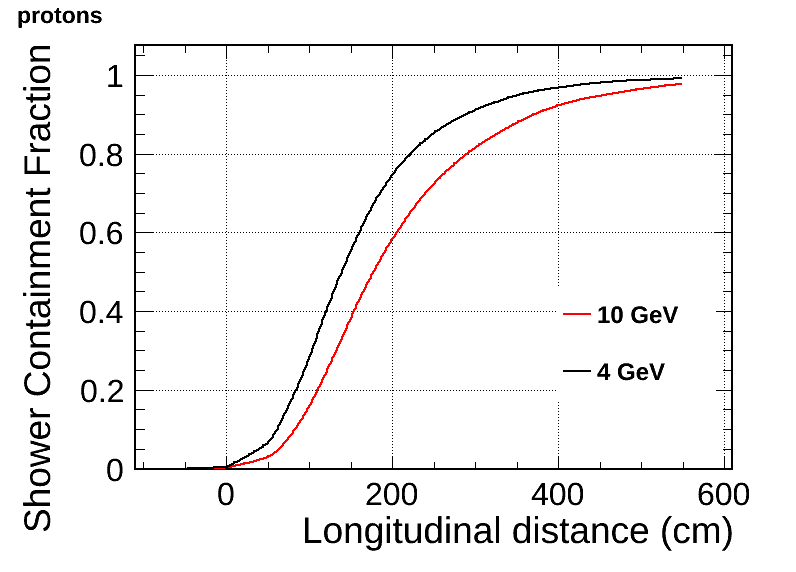
\includegraphics[width=0.49\textwidth,height=4.9cm]{protons_lcont_overlay}&
   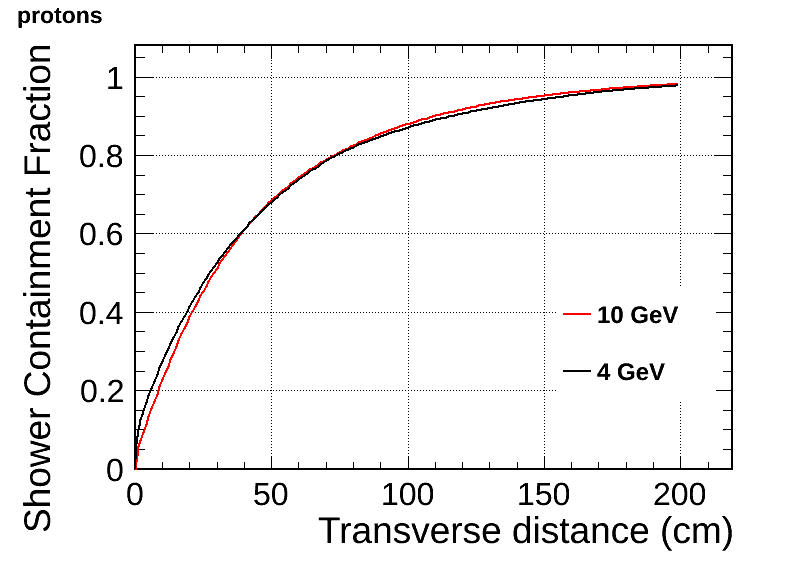
\includegraphics[width=0.49\textwidth,height=4.9cm]{protons_wcont_overlay}\\
  \end{tabular}
\end{cdrfigure}

\item $dQ/dx$ and $dQ/dx$ vs. range for charge particles (protons, pion, muon, kaon)

%\fixme{I did not remove kaon words, but are they still on the (realistic) list? Please, remove if not.}


\item Fraction of true energy deposited by interacting charge particles 


\end{itemize}

%%%%%%%%%%%%%%%%%%%%%%%%%%%%%%%%%%%%%%%%%%%%%%
%%%---\section{Evaluation of event reconstruction performance}


%In the following, we define the goals that we aim to achieve regarding the TPC electronic noise and signal processing.
This section describes the requirements for the TPC electronic noise and signal processing.

\begin{itemize}
\item The number of unusable channels is required to be smaller than 1\%: \\

All the past or current large LArTPC experiments (ICARUS, MicroBooNE, and DUNE-35ton) have suffered from a sizable
number of unusable channels ($>$ 10\%) for %due to various reasons such as high noise, dead electronics, and disconnected wires. At the same time, each of the experiment achieved successes in reductions of the problems that cause some of the wires to be unusable. 
For example, ICARUS has no disconnected wires. In LAriat, all cold electronics channels ($\sim$ 500) are live and achieve the expected $\sim$400 electrons equivalent noise charge (ENC). In the ATLAS LAr calorimeter, only about 0.1\% of the cold electronics channels are unusable. 
In MicroBooNE, the ENC after software noise filtering is about 400 electrons, which is consistent with the design specification of the cold electronics. Also, all the major sources of electronic noise
have been identified, and hardware solutions are in order. Therefore, with careful and systematic quality assurance and controls, it is possible to reduce the total number of unusable channels
by at least one order of magnitude. This is one of the primary goals of ProtoDUNE.

\fixme{the above is not clear. 
It needs a progression something like this:
`All these detectors have had channel problems. Problems have been identified and are fixed. From this we know we can reduce unusable channels by order of magnitude.' The sentence about successes is confusing: success after fixing? Or success in other areas? DONE(?)
}




\item The overall signal calibration process is required to be validated: \\
The goal of the signal calibration process is to recover the number of ionized electrons based on
the digitized TPC waveform; this is the first step in the overall event reconstruction. It is crucial to validate that such a procedure is robust. 
This validation can be achieved by comparing the images from the raw digits with the images after the deconvolution procedure.

\end{itemize}




%%%%%%%%%%%%%%%%%%%%%%%%%%%%%%%%%%%%%%%%%%%%%%
%%%---\section{Particle interactions and cross sections}





%%%%%%%%%%%%%%%%%%%%%%%%%%%%%%%%%%%%%%%%%%%%%%%%%
\section{Detector engineering validation}

One of the primary goals of the ProtoDUNE-SP experiment is to validate the engineering design of the elements proposed for the 10 kt DUNE single-phase detector. ProtoDUNE-SP is designed so that it will provide information on the actual far detector performance in as close a possible a configuration to the actual far detector layout as possible given the practical considerations imposed by time, space, and cost. To achieve this the cold components are wherever possible identical to the components proposed for the far detector. 

As an example the APA modules are full-scale pre-production modules for the far detector. The full-scale APA modules have 20 front end readout board instrumenting each and 10 integrated photon detector paddles. The ground connections between the electronics, the APA mechanical structure, the photon detectors, and the detector support structure will be as proposed for DUNE SP detector. ProtoDUNE-SP is instrumented with three APAs along each wall which will test that there is no cross talk between the middle APA and the neighboring ones. However, there are some practical limitations which required compromise in the ProtoDUNE design. The far detector is designed with a 12 m high TPC based on a two APA high layout where the bottom APA is hung from the top. Given the space available and generally the cost of the cryogenic infrastructure it is not practical to have a 12 m high test experiment. For these reasons ProtoDUNE-SP is designed with a single APA high TPC. The collaboration will test separately the mechanical process of installing the two APA detector configuration along with the related cabling.

The readout electronics is designed based on the far detector cryogenic front end pre-amp/shaper chip and ADC.  The dedicated ASIC for serializing the data and providing a 1GB/s link is not yet available so an FPGA emulating its functionality will be used and is mounted on a dedicated mezzanine board. It should be pointed out that all the analog components, the conversion to digital and the grounding/power distribution for the final electronics can be tested in this configuration. 

ProtoDUNE-SP will be the largest experiment to take data with the cold electronics allowing high statistic detailed studies of the performance. In the event further optimization of the ASICs are required based on the ProtoDUNE-SP findings, this can be implemented before production start in 2020. As there is no charge amplification in the liquid in the Single-Phase detector, the electronics must be extremely sensitive which makes the grounding and shielding critical. The ProtDUNE-SP experiment is designed to be as close to the far detector grounding as practical. The building ground in ENH1 with all the rebar in the concrete floor interconnected and then this network connected to the building ground bus should provide a fairly good ground for ProtoDUNE. The cryostat itself is isolated from the building ground and all the mechanical/electrical connections have dielectric breaks. At the far site the detector is a mile underground in a very dry mine so one expects better isolation from the environment, but the ProtoDUNE will test the ground isolation and shielding under conservative conditions.

The field cage and cathode planes are full-scale prototypes of the final far detector elements. As the ProtoDUNE-SP detector is designed with full-scale field cages the maximum drift distance and corresponding high voltage will be the same as planned for the far detector. This allows ProtoDUNE to use the same high voltage feed thru as DUNE-SP and the drift field configuration that is planned for the far detector. The cryostat dimensions are selected to be the same as the Dual-Phase cryostat in order to only need to design one cryostat and cryogenic system. In order to fit in the cryostat the wall to cathode plane distance is slightly smaller than in the far detector making this setup a conservative test of the HV design. The ground planes above and below the detector make the actual mechanical geometry inside the cryostat on the top and bottom irrelevant for issues related to high voltage. This preserves the freedom to tailor the far detector cryogenics system as needed to optimize the purification without compromising the validity of the ProtoDUNE test. 

Testing these components under nominal operating conditions is extremely important as this is the first instance of LArTPCs operating with a resistive cathode or the field cage construction with metal profiles and fiberglass I-beam support. In the event ProtoDUNE-SP wishes a second run with a shorter drift distance in order to reduce the effects of space charge the FC can be shortened to 2.5 m maximum drift distance.

ProtoDUNE offers a unique platform to validate and possibly optimize the cryogenic design for DUNE. The DUNE 35t prototype was the first membrane cryostat to achieve high purity operation, but it was limited to roughly 3 ms $e^-lifetime$. This is substantially worse than the MicroBooNE experiment's  $\sim$10 ms or the lifetimes seen at ICARUS at the end of its last run. 

There are several possible causes for a shorter electron lifetime.  A third of the 35t cryostat roof is covered with a hatch that is not insulated but designed with radiation shields. As the dominant source of contamination is the transfer of impurities in the gas ullage to the liquid, the gas circulation in the ullage and the impact of the hatch are important factors in the cryostat/cryogenics design. The purity monitors inside the 35t cryostat also indicated that the liquid was not well mixed with substantially higher purity at the bottom of the cryostat indicating that the liquid feed and temperature need to be optimized.  

The ProtoDUNE-SP cryostat design does not have a hatch for the detector installation instead a temporary construction opening (TCO) is used (similar to the Dual-Phase cryostat). The Single-Phase detector moved to this option after the difficulties encountered in the mechanical design of the hatch for the 1x1x3 cryostat and based on the recommendations from the cryostat design team.  This will also eliminate one potential source of contamination to the liquid argon. It should be pointed out that with a 3 ms lifetime and a 2.25 ms maximum drift time roughly half the charge generated near the cathode is lost before it reaches the anode. Efforts to improve the electron lifetime will improve the detector performance.  Cryogenic design improvements are that the Proto-DUNE SP detector will not have a hatch in the ullage, all cryostat penetrations will be designed with gas purge to prevent contaminates from migrating from warm surfaces to the ullage volume, and the cryostat/cryogenic system will be modeled to understand the liquid and gas flows inside the cryostat. ProtoDUNE-SP will provide an excellent test bed to prove the cryogenic design for DUNE. 

The installation process has many similarities to the far detector installation but also many differences. Both installation plans now call for inserting the equipment through a TCO. ProtoDUNE-SP will prototype the tooling and procedures for transporting an APA and transferring to to a suspended rail system. Similarly the assembly and transport of the cathode planes and top/bottom field cages will be developed. What will not be tested is the hanging of one APA from the other and the difference in moving a 12 m stack instead of one 6 m module. Likewise the CPA is only 6 m tall instead of 12 m. One major change in the installation was forced by the need to install the end walls with the TCO closure and the beam interface. Due to the tight space inside the cryostat the rail structure on which the detector is hung will most likely be different for the final detector. However the experience in installing the ProtoDUNE-SP detector will be invaluable in planning the DUNE far detector installation. 

Finally one significant difference between the ProtoDUNE-SP detector and the single-phase far detector is the integration of the test beam. This requires a penetration into the cryostat and a liquid argon displacement plug bridging the gap between the membrane cryostat wall and the detector field cage. As this element bridges the high voltage careful design is required. To insure that the displacement plug does not compromise the ProtoDUNE-SP operation a dedicated HV test at FNAL is planned which will test the final beam plug in the exact field configuration planned for ProtoDUNE.


%%%%%%%%%%%%%%%%%%%%%%%%%%%%%%%%%%%%%%%%%%%%%%
%%%---\section{Installation validation}




